% =====================================================================
%  fig_method_architecture.tex
%  Thermal Lift -- method / system architecture figure (AAAI figure*)
%
%  Standalone, self-contained: compile with
%      pdflatex fig_method_architecture.tex
%
%  Story: under a calibrated forward model with NO HR ground truth,
%  show (i) physics/forward model, (ii) how multi-frame evidence enters
%  the network, (iii) residual-over-observation parameterization that
%  makes "keep the observation" the default solution, plus the three
%  guiding questions Q1 (information exists) / Q2 (delivered) / Q3 (faithful).
%
%  Claim boundary: 2x contour-level enhancement (5 um sample, 10 um
%  Nyquist period) -- NOT 4x, NOT 5 um resolution, NOT temperature metrology.
% =====================================================================
\documentclass[border=8pt]{standalone}

\usepackage{mathptmx}      % Times text + math (CVPR/AAAI serif)
\usepackage{amsmath}
\usepackage{pifont}        % \ding{55} = cross mark
\usepackage{tikz}
\usetikzlibrary{positioning,arrows.meta,fit,backgrounds,calc}

% ---------------------------------------------------------------- colours
\definecolor{physfill}{HTML}{E6ECF4}  % cold gray-blue (physical lane)
\definecolor{physdraw}{HTML}{4C6E96}
\definecolor{learndraw}{HTML}{454545} % neutral dark gray (learning path)
\definecolor{resfill}{HTML}{FCE7D2}   % light warm orange (residual focus)
\definecolor{resdraw}{HTML}{D9772F}   % warm orange accent
\definecolor{clsfill}{HTML}{E3F0E6}   % muted green (classical anchors)
\definecolor{clsdraw}{HTML}{4F9266}
\definecolor{evalfill}{HTML}{DEE9F5}  % light steel blue (evaluation)
\definecolor{evaldraw}{HTML}{4C72B0}
\definecolor{qfill}{HTML}{EFEAF6}     % light lavender (three questions)
\definecolor{qdraw}{HTML}{7B6BA8}
\definecolor{ablgray}{HTML}{9A9A9A}   % ablated / falsified
\definecolor{notered}{HTML}{B4474B}   % cautionary note
\definecolor{lanebg}{HTML}{F7F8FA}
\definecolor{lanedraw}{HTML}{C9CFD8}

% ---------------------------------------------------------------- text helpers
\newcommand{\hd}[1]{{\small\bfseries #1}}                          % component title (~9pt)
\newcommand{\nt}[1]{{\scriptsize #1}}                              % annotation (~7pt)
\newcommand{\pr}[1]{{\scriptsize\itshape\textcolor{physdraw}{#1}}} % prior caveat
\newcommand{\bad}[1]{{\scriptsize\textcolor{notered}{#1}}}         % red caution note
\newcommand{\xm}{\textcolor{notered}{\ding{55}}}
\newcommand{\um}{\ensuremath{\mu}m}          % micrometre, safe in text & math
\newcommand{\dgr}{\ensuremath{{}^\circ}}      % degree, safe in text & math

% ---------------------------------------------------------------- styles
\tikzset{
  block/.style   ={rounded corners=2pt, draw, line width=0.6pt, inner sep=3.5pt, align=left},
  phys/.style    ={block, fill=physfill, draw=physdraw},
  learn/.style   ={block, fill=white,    draw=learndraw},
  res/.style     ={block, fill=resfill,  draw=resdraw, line width=1.3pt},
  cls/.style     ={block, fill=clsfill,  draw=clsdraw},
  eval/.style    ={block, fill=evalfill, draw=evaldraw},
  forge/.style   ={block, fill=physfill, draw=physdraw, densely dashed},
  callout/.style ={block, fill=physfill!55, draw=physdraw, dashed, rounded corners=6pt},
  loss/.style    ={block, fill=white, draw=learndraw, densely dashed},
  ablated/.style ={block, fill=black!7, draw=ablgray, dashed, text=black!75},
  qtag/.style    ={rounded corners=3pt, draw=qdraw, fill=qfill, line width=0.9pt,
                   inner sep=3pt, align=left, font=\scriptsize},
  df/.style      ={-{Stealth[length=4pt]}, line width=0.7pt, draw=black!72},
  sup/.style     ={-{Stealth[length=3.5pt]}, line width=0.6pt, draw=learndraw, densely dashed},
  prior/.style   ={-{Stealth[length=3.5pt]}, line width=0.6pt, draw=physdraw, dotted},
  ch5/.style     ={-{Stealth[length=5pt]}, line width=1.7pt, draw=resdraw},
  abl/.style     ={-{Stealth[length=3.5pt]}, line width=0.6pt, draw=ablgray, dashed},
  lead/.style    ={draw=qdraw, line width=0.5pt, densely dotted},
  lanelabel/.style={font=\small\bfseries, text=black!72, anchor=north west},
}

\begin{document}
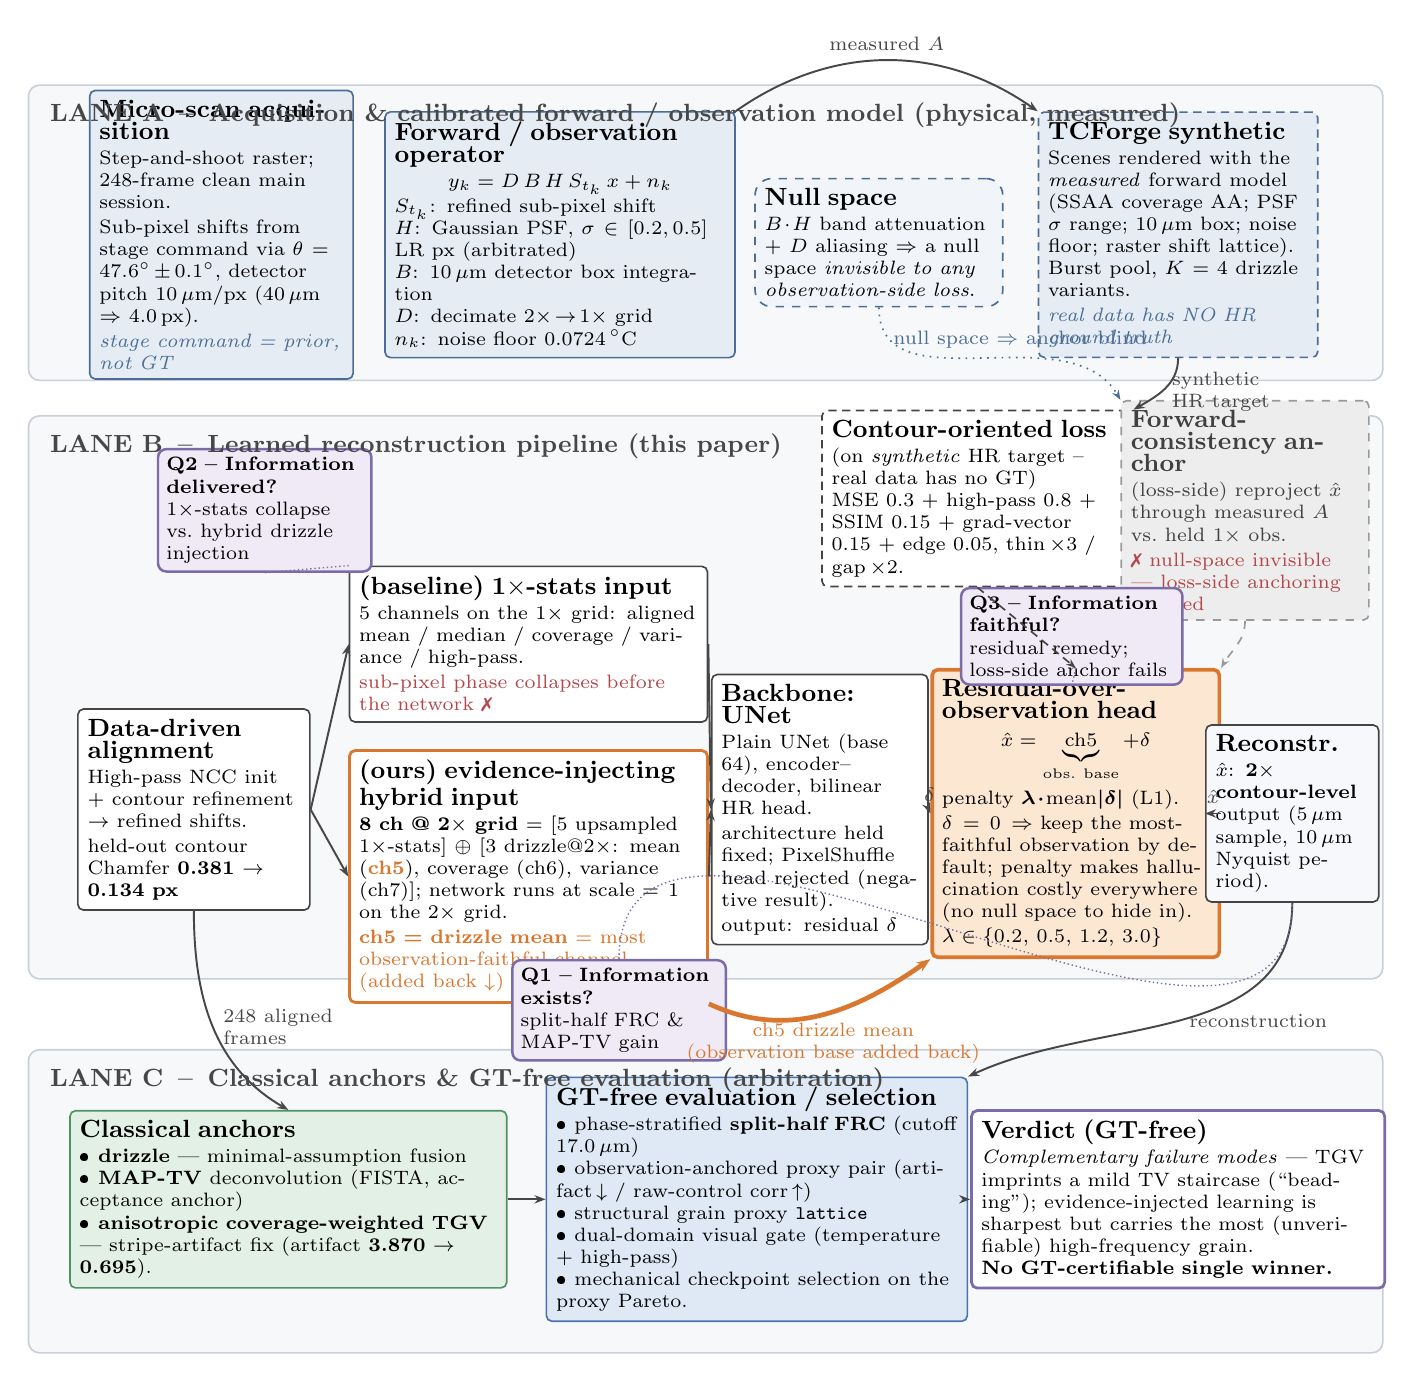
\begin{tikzpicture}[font=\scriptsize]

% =================================================================
%  LANE A  -- acquisition + calibrated forward / observation model
% =================================================================
\node[phys, text width=3.1cm] (acq) at (2.10,11.40){%
  \hd{Micro-scan acquisition}\\[1pt]
  \nt{Step-and-shoot raster; 248-frame clean main session.}\\[1pt]
  \nt{Sub-pixel shifts from stage command via $\theta=47.6\dgr\!\pm\!0.1\dgr$, detector pitch 10\,\um/px (40\,\um\ $\Rightarrow$ 4.0\,px).}\\[1pt]
  \pr{stage command = prior, not GT}%
};

\node[phys, text width=4.2cm] (fwd) at (6.40,11.40){%
  \hd{Forward / observation operator}\\[1pt]
  {\centering$y_k = D\,B\,H\,S_{t_k}\,x + n_k$\par}\vspace{1pt}
  \nt{$S_{t_k}$: refined sub-pixel shift\\
      $H$: Gaussian PSF, $\sigma\in[0.2,0.5]$ LR px (arbitrated)\\
      $B$: 10\,\um\ detector box integration\\
      $D$: decimate $2\times\!\rightarrow\!1\times$ grid\\
      $n_k$: noise floor 0.0724\,\dgr C}%
};

\node[callout, text width=2.9cm] (nullsp) at (10.45,11.30){%
  \hd{Null space}\\[1pt]
  \nt{$B\!\cdot\!H$ band attenuation $+$ $D$ aliasing $\Rightarrow$ a null space \emph{invisible to any observation-side loss}.}%
};

\node[forge, text width=3.3cm] (forge) at (14.25,11.40){%
  \hd{TCForge synthetic}\\[1pt]
  \nt{Scenes rendered with the \emph{measured} forward model (SSAA coverage AA; PSF $\sigma$ range; 10\,\um\ box; noise floor; raster shift lattice). Burst pool, $K=4$ drizzle variants.}\\[1pt]
  \pr{real data has NO HR ground truth}%
};

% =================================================================
%  LANE B  -- learned reconstruction pipeline  (this paper, core)
% =================================================================
\node[learn, text width=2.7cm] (align) at (1.75,4.10){%
  \hd{Data-driven alignment}\\[1pt]
  \nt{High-pass NCC init $+$ contour refinement $\rightarrow$ refined shifts.}\\[1pt]
  \nt{held-out contour Chamfer \textbf{0.381 $\rightarrow$ 0.134 px}}%
};

\node[learn, text width=4.3cm] (inbase) at (6.00,6.20){%
  \hd{(baseline) 1$\times$-stats input}\\[1pt]
  \nt{5 channels on the 1$\times$ grid: aligned mean / median / coverage / variance / high-pass.}\\[1pt]
  \bad{sub-pixel phase collapses before the network \xm}%
};

\node[learn, text width=4.3cm, draw=resdraw, line width=1.0pt] (inours) at (6.00,3.25){%
  \hd{(ours) evidence-injecting hybrid input}\\[1pt]
  \nt{\textbf{8 ch @ 2$\times$ grid} $=$ [5 upsampled 1$\times$-stats] $\oplus$ [3 drizzle@2$\times$: mean (\textbf{\textcolor{resdraw}{ch5}}), coverage (ch6), variance (ch7)]; network runs at scale $=1$ on the 2$\times$ grid.}\\[1pt]
  {\scriptsize\textcolor{resdraw}{\textbf{ch5 = drizzle mean} = most observation-faithful channel (added back $\downarrow$)}}%
};

\node[learn, text width=2.5cm] (unet) at (9.70,4.10){%
  \hd{Backbone: UNet}\\[1pt]
  \nt{Plain UNet (base 64), encoder--decoder, bilinear HR head.}\\[1pt]
  \nt{architecture held fixed; PixelShuffle head rejected (negative result).}\\[1pt]
  \nt{output: residual $\delta$}%
};

\node[res, text width=3.4cm] (resid) at (12.95,4.05){%
  \hd{Residual-over-observation head}\\[2pt]
  {\centering$\hat{x} = \underbrace{\text{ch5}}_{\text{obs.\ base}} + \delta$\par}\vspace{2pt}
  \nt{penalty $\boldsymbol{\lambda\!\cdot\!\text{mean}|\delta|}$ (L1).}\\[1pt]
  \nt{$\delta=0\Rightarrow$ keep the most-faithful observation by default; penalty makes hallucination costly everywhere (no null space to hide in).}\\[1pt]
  \nt{$\lambda\in\{0.2,\,0.5,\,1.2,\,3.0\}$}%
};

\node[learn, text width=1.95cm, fill=physfill!35] (out) at (15.70,4.05){%
  \hd{Reconstr.}\\[1pt]
  \nt{$\hat{x}$: \textbf{2$\times$ contour-level} output (5\,\um\ sample, 10\,\um\ Nyquist period).}%
};

% -- supervision row (above main path) --------------------------------
\node[loss, text width=3.7cm] (closs) at (11.70,8.05){%
  \hd{Contour-oriented loss}\\[1pt]
  \nt{(on \emph{synthetic} HR target -- real data has no GT)\\
      MSE 0.3 $+$ high-pass 0.8 $+$ SSIM 0.15 $+$ grad-vector 0.15 $+$ edge 0.05, thin\,$\times$3 / gap\,$\times$2.}%
};

\node[ablated, text width=2.9cm] (fanchor) at (15.10,7.90){%
  \hd{Forward-consistency anchor}\\[1pt]
  \nt{(loss-side) reproject $\hat{x}$ through measured $A$ vs.\ held 1$\times$ obs.}\\[1pt]
  \bad{\xm\ null-space invisible --- loss-side anchoring falsified}%
};

% =================================================================
%  LANE C  -- classical anchors + GT-free evaluation (arbitration)
% =================================================================
\node[cls, text width=5.3cm] (classic) at (2.95,-0.85){%
  \hd{Classical anchors}\\[1pt]
  \nt{\textbullet\ \textbf{drizzle} --- minimal-assumption fusion\\
      \textbullet\ \textbf{MAP-TV} deconvolution (FISTA, acceptance anchor)\\
      \textbullet\ \textbf{anisotropic coverage-weighted TGV} --- stripe-artifact fix (artifact \textbf{3.870 $\rightarrow$ 0.695}).}%
};

\node[eval, text width=5.1cm] (eval) at (8.90,-0.85){%
  \hd{GT-free evaluation / selection}\\[1pt]
  \nt{\textbullet\ phase-stratified \textbf{split-half FRC} (cutoff 17.0\,\um)\\
      \textbullet\ observation-anchored proxy pair (artifact\,$\downarrow$ / raw-control corr\,$\uparrow$)\\
      \textbullet\ structural grain proxy \texttt{lattice}\\
      \textbullet\ dual-domain visual gate (temperature $+$ high-pass)\\
      \textbullet\ mechanical checkpoint selection on the proxy Pareto.}%
};

\node[block, fill=white, draw=qdraw, line width=1.0pt, text width=5.0cm] (verdict) at (14.25,-0.85){%
  \hd{Verdict (GT-free)}\\[1pt]
  \nt{\emph{Complementary failure modes} --- TGV imprints a mild TV staircase (``beading''); evidence-injected learning is sharpest but carries the most (unverifiable) high-frequency grain.\\
      \textbf{No GT-certifiable single winner.}}%
};

% =================================================================
%  three guiding questions (unified lavender tags)
% =================================================================
\node[qtag, text width=2.5cm] (q2) at (2.65,7.90){\textbf{Q2 -- Information delivered?}\\ 1$\times$-stats collapse vs.\ hybrid drizzle injection};
\node[qtag, text width=2.6cm] (q3) at (12.90,6.30){\textbf{Q3 -- Information faithful?}\\ residual remedy; loss-side anchor fails};
\node[qtag, text width=2.5cm] (q1) at (7.15,1.55){\textbf{Q1 -- Information exists?}\\ split-half FRC \& MAP-TV gain};

% =================================================================
%  connectors
% =================================================================
% Lane A internal: forward model feeds the synthetic renderer (arc over null space)
\draw[df] (fwd.north east) to[out=35,in=145]
      node[above, font=\scriptsize, text=black!72]{measured $A$} (forge.north west);

% Lane A -> Lane B : synthetic HR target into the loss
\draw[df] (forge.south) to[out=-90,in=30]
      node[pos=0.55,right,font=\scriptsize,text=black!72,align=left]{synthetic\\HR target} (closs.north east);

% null space makes the loss-side anchor blind (echoes Q3)
\draw[prior] (nullsp.south) to[out=-90,in=120]
      node[pos=0.62,above,font=\scriptsize,text=physdraw]{null space $\Rightarrow$ anchor blind} (fanchor.north west);

% main learned data flow
\draw[df] (align.east) -- (inbase.west);
\draw[df] (align.east) -- (inours.west);
\draw[df] (inbase.east) -- (unet.west);
\draw[df] (inours.east) -- (unet.west);
\draw[df] (unet.east) -- node[above,font=\scriptsize,text=black!72]{$\delta$} (resid.west);
\draw[df] (resid.east) -- node[above,font=\scriptsize,text=black!72]{$\hat{x}$} (out.west);

% ch5 evidence-injection highlight (routed below the main row)
\draw[ch5] (inours.south east) to[out=-25,in=215]
      node[below,pos=0.55,font=\scriptsize,text=resdraw,align=center]{ch5 drizzle mean\\(observation base added back)}
      (resid.south west);

% supervision (loss / anchor -> reconstruction head)
\draw[sup] (closs.south) -- (resid.north);
\draw[abl] (fanchor.south) to[out=-90,in=60] (resid.north east);

% reconstruction + aligned frames feed evaluation
\draw[df] (align.south) to[out=-90,in=150]
      node[pos=0.5,right,font=\scriptsize,text=black!72,align=left]{248 aligned\\frames} (classic.north);
\draw[df] (out.south) to[out=-90,in=25]
      node[pos=0.5,right,font=\scriptsize,text=black!72]{reconstruction} (eval.north east);
\draw[df] (classic.east) -- (eval.west);
\draw[df] (eval.east) -- (verdict.west);

% Q tag leaders
\draw[lead] (q2.south) -- (inbase.north west);
\draw[lead] (q3.south) -- (resid.north);
\draw[lead] (q1.north) to[out=90,in=-90] (out.south);

% =================================================================
%  lane backgrounds + titles (drawn behind everything)
% =================================================================
\begin{scope}[on background layer]
  \fill[lanebg, draw=lanedraw, line width=0.6pt, rounded corners=4pt]
        (-0.35, 9.55) rectangle (16.85,13.30);
  \fill[lanebg, draw=lanedraw, line width=0.6pt, rounded corners=4pt]
        (-0.35, 1.95) rectangle (16.85, 9.10);
  \fill[lanebg, draw=lanedraw, line width=0.6pt, rounded corners=4pt]
        (-0.35,-2.80) rectangle (16.85, 1.05);
\end{scope}

\node[lanelabel] at (-0.20,13.20){LANE A\, --\, Acquisition \& calibrated forward / observation model (physical, measured)};
\node[lanelabel] at (-0.20, 9.00){LANE B\, --\, Learned reconstruction pipeline (this paper)};
\node[lanelabel] at (-0.20, 0.95){LANE C\, --\, Classical anchors \& GT-free evaluation (arbitration)};

\end{tikzpicture}
\end{document}
